\documentclass[conference]{IEEEtran}

\usepackage[T1]{fontenc}
\usepackage[utf8]{inputenc}
\usepackage{babel}
\babelprovide[main,import]{portuguese}
\usepackage{amsmath}
\usepackage{cite}
\usepackage{booktabs,tabularx}
\usepackage{tikz}
\usetikzlibrary{arrows.meta,positioning}
\usepackage{xurl}
\usepackage[hidelinks]{hyperref}
\hypersetup{pdftitle={Simulação de uma missão de busca e salvamento em Marte}}

\addto\captionsportuguese{%
  \renewcommand{\abstractname}{Resumo}%
  \renewcommand{\IEEEkeywordsname}{Palavras-chave}%
  \renewcommand{\refname}{Referências}%
  \renewcommand{\figurename}{Fig.}%
  \renewcommand{\tablename}{Tabela}%
}

\title{Simulação de uma missão de busca e salvamento em Marte}

% Completar o nome do segundo autor e confirmar a afiliação antes da entrega.
\author{\IEEEauthorblockN{Alexandre Coelho e Gonçalo Noronha}
\IEEEauthorblockA{Instituto Superior de Engenharia do Porto\\
Porto, Portugal}}

\begin{document}
\maketitle

\begin{abstract}
Este trabalho apresenta um sistema multirrobótico simulado em que um drone X500 procura o módulo de pouso Pathfinder e fornece a sua posição a um rover Perseverance. O drone sobrevoa a área de busca com o autopilot PX4 e utiliza um detetor YOLO para identificar o alvo nas imagens da câmara. A deteção é projetada sobre o terreno e a posição estimada é publicada num tópico ROS2. O rover subscreve esse tópico, calcula um ponto de aproximação junto do alvo e navega até esse ponto usando a pose disponibilizada pelo Gazebo. Num ensaio integrado, os dois robôs executaram esta sequência autonomamente. A avaliação foi qualitativa e incidiu num único ponto de interesse, num percurso em que a deteção de obstáculos não foi acionada.
\end{abstract}

\begin{IEEEkeywords}
Sistemas multirrobóticos, ROS2, Gazebo, PX4, YOLO, navegação autónoma.
\end{IEEEkeywords}

\section{Problema}
\subsection{Contexto e objetivo}

A missão Mars~2020 da NASA levou o rover Perseverance a Marte \cite{farley2020,nasa-perseverance}. A missão incluiu o Ingenuity, um helicóptero experimental transportado pelo rover \cite{balaram2021,nasa-ingenuity}. A combinação de um veículo aéreo com um veículo terrestre inspirou o cenário simulado deste trabalho. Neste cenário, o módulo de pouso da missão Mars Pathfinder foi representado como o objeto a localizar \cite{golombek1997,nasa-pathfinder}.

O requisito central do projeto de Redes de Sensores Distribuídos era pôr dois robôs a operar e a comunicar entre si. O grupo definiu uma missão em que o robô aéreo recolhe informação sobre um alvo e o rover usa essa informação para decidir para onde se deslocar. A proposta inicial previa que o Ingenuity identificasse vários pontos de interesse, publicasse uma lista ordenada por prioridade e que o Perseverance planeasse sucessivamente a deslocação entre esses pontos. O âmbito demonstrado foi reduzido a um único ponto de interesse (POI) e a função de reconhecimento aéreo passou para o X500.

\subsection{Requisitos da missão demonstrada}

O X500 devia sobrevoar a área de busca, identificar o Pathfinder e disponibilizar a sua posição. O Perseverance devia receber essa posição e chegar autonomamente a um ponto próximo do objeto, com afastamento suficiente para evitar contacto com o modelo. A integração devia permitir executar a sequência sem introduzir manualmente as coordenadas do alvo durante o ensaio.

\section{Solução}
\subsection{Cenário e componentes reutilizados}

O cenário reutilizou o terreno marciano e o modelo do rover Perseverance do pacote \texttt{spaceros\_gz\_demos} \cite{spaceros-demo}. Para representar o módulo de aterragem Mars Pathfinder, foi descarregado do 3D Warehouse do SketchUp o modelo \textit{Mars Pathfinder Lander (HIGH Detail)} \cite{pathfinder-mesh}. A malha, em formato COLLADA (\texttt{.dae}), foi organizada na pasta \texttt{mars\_pathfinder}, juntamente com os ficheiros \texttt{model.config} e \texttt{model.sdf}. No cenário, o Pathfinder foi colocado como um alvo estático dentro da área de busca do X500.
A simulação foi executada com ROS2 Jazzy e Gazebo Harmonic \cite{macenski2022,ros-jazzy,koenig2004,gazebo}. O mundo e os modelos foram descritos em SDFormat \cite{sdformat}. A ponte \texttt{ros\_gz\_bridge} disponibilizou ao ROS2 a pose e os dados da câmara de profundidade do rover e encaminhou para o Gazebo os comandos de velocidade \cite{bridge}. Os nós de controlo foram desenvolvidos em C++ com \texttt{rclcpp} \cite{rclcpp}.
\subsection{X500 e localização do Pathfinder}

\textit{Controlo de voo.}
Após muitos problemas com Ingenuity e as suas Swashplats, mudou-se para o X500, que contem o seu próprio autopiloto através de PX4. Este percorre a área de busca seguindo pontos de passagem. O nó de missão envia referências de posição ao PX4 em modo \textit{Offboard}. O autopiloto trata do controlo de voo a partir dessas referências \cite{px4-offboard}. Na configuração de arranque do X500, o Micro XRCE-DDS Agent liga o cliente PX4 à rede DDS. A interface disponibiliza nos tópicos \texttt{/fmu/out/} os dados de posição local e atitude usados para localizar o alvo \cite{px4-ros2,xrce-agent}.

\textit{Deteção na imagem.}
O YOLO processa cada imagem da câmara e estima caixas delimitadoras e pontuações de confiança para as classes detetadas \cite{yolo}. Neste projeto, a classe de interesse é o Pathfinder, mas facilmente pode se adicionar outros objetos. A deteção indica onde o objeto aparece na imagem. O passo seguinte usa esse ponto em píxeis para estimar a posição física do alvo.

\textit{Projeção para o mundo.}
No pacote \texttt{x500\_control}, o nó \texttt{PoiLocator} recebe a deteção e usa a posição e a atitude provenientes do PX4 para transformar o raio de observação para o referencial do mundo. A estimativa corresponde à interseção desse raio com a representação da elevação do terreno. A transformação tem em conta a convenção NED (norte, este, baixo) usada pelo PX4 e a convenção ENU (este, norte, cima) usada na representação do mundo \cite{px4-ros2}. Deteções sucessivas que resultem em posições próximas permitem confirmar o alvo. O ponto confirmado é publicado em \texttt{/x500/poi} como uma mensagem \texttt{geometry\_msgs/msg/PointStamped}, com o referencial \texttt{world}. O nó pode disponibilizar as estimativas intermédias em \texttt{/x500/blob\_world}, enquanto o rover recebe o ponto confirmado no tópico de missão \cite{point-stamped}.

\subsection{Perseverance e navegação terrestre}

\textit{Posição e acionamento.}
O controlador terrestre utiliza a pose de referência do Gazebo (\textit{ground truth}), publicada pelo \texttt{OdometryPublisher} e disponibilizada em ROS2 no tópico \url{/perseverance/ground_truth/odometry} como \texttt{nav\_msgs/msg/Odometry} \cite{odom-publisher,odometry}. O grupo reconfigurou o plugin \texttt{DiffDrive} para comandar as seis rodas. O modelo inicial acionava apenas as duas rodas dianteiras.

\textit{Aproximação ao alvo.}
O nó subscreve \texttt{/x500/poi} e calcula um destino nas imediações do Pathfinder, com um afastamento em relação ao ponto recebido. O controlo usa a diferença de posição no plano horizontal. Seja $(x,y)$ a posição do rover, $\psi$ a sua orientação em torno do eixo vertical e $(x_a,y_a)$ o ponto de aproximação. A distância ao destino e o erro de orientação são dados por
\begin{align}
d &= \sqrt{(x_a-x)^2+(y_a-y)^2}, \\
\psi_a &= \operatorname{atan2}(y_a-y, x_a-x), \\
e_\psi &= \operatorname{atan2}\bigl(\sin(\psi_a-\psi),\,
                                   \cos(\psi_a-\psi)\bigr).
\end{align}
A velocidade angular corrige o erro de orientação. O controlador autoriza o avanço quando o rover está alinhado dentro da tolerância angular e termina a aproximação quando a distância ao destino fica dentro da tolerância de chegada. O nó do pacote \url{perseverance_navigation} publica os comandos de velocidade linear e angular em \url{/perseverance/cmd_vel} através de mensagens \texttt{geometry\_msgs/msg/Twist} \cite{twist}.

\textit{Deteção de obstáculos.}
O nó de navegação recebe a nuvem de pontos da câmara de profundidade e verifica se há pontos suficientes numa região à frente do rover. A lógica pode ordenar a paragem perante um obstáculo nessa região. A interface de profundidade utiliza mensagens \texttt{sensor\_msgs/msg/PointCloud2} \cite{pointcloud}.

\begin{figure}[!t]
\centering
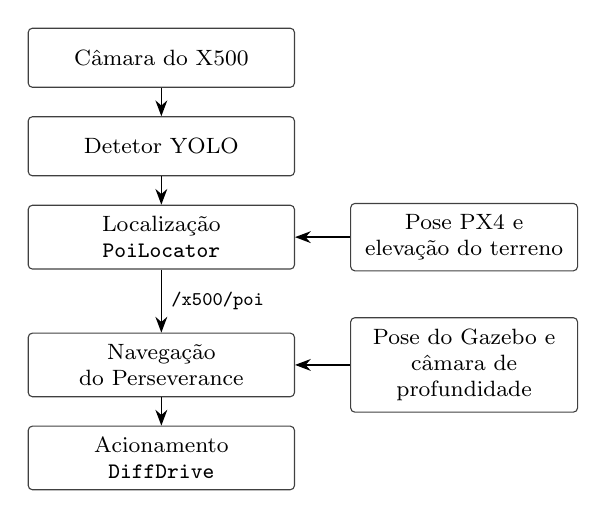
\begin{tikzpicture}[
  block/.style={draw=black!75, rounded corners=1.5pt, align=center,
    inner sep=4pt, minimum height=7.5mm, text width=31mm, font=\footnotesize},
  side/.style={block,text width=26mm},
  flow/.style={-{Stealth[length=2mm]},semithick},
  node distance=3.6mm
]
  \node[block] (cam) {Câmara do X500};
  \node[block,below=of cam] (det) {Detetor YOLO};
  \node[block,below=of det] (poi) {Localização\\\texttt{PoiLocator}};
  \node[block,below=8mm of poi] (rover) {Navegação\\do Perseverance};
  \node[block,below=of rover] (drive) {Acionamento\\\texttt{DiffDrive}};
  \node[side,right=7mm of poi] (px) {Pose PX4 e\\elevação do terreno};
  \node[side,right=7mm of rover] (gz) {Pose do Gazebo e\\câmara de profundidade};
  \draw[flow] (cam) -- (det);
  \draw[flow] (det) -- (poi);
  \draw[flow] (px) -- (poi);
  \draw[flow] (poi) -- node[right,font=\scriptsize\ttfamily] {/x500/poi} (rover);
  \draw[flow] (gz) -- (rover);
  \draw[flow] (rover) -- (drive);
\end{tikzpicture}
\caption{Fluxo de informação desde a deteção aérea até ao acionamento do rover.}
\label{fig:fluxo}
\end{figure}

\subsection{Integração entre os robôs}

A Fig.~\ref{fig:fluxo} mostra o fluxo de informação entre a deteção aérea e o controlo terrestre. A publicação do ponto num tópico ROS~2 separa a produção da estimativa do seu uso pelo rover \cite{ros-topics}. O referencial comum permite interpretar a posição do alvo e a pose do Perseverance no mesmo sistema de coordenadas. As coordenadas são disponibilizadas pelo tópico durante a operação, sem exportação para CSV no fluxo final.

\section{Resultados}
\subsection{Ensaio integrado}

O ensaio integrado percorreu a sequência completa numa única execução. O X500 sobrevoou a área, identificou o Pathfinder e publicou as coordenadas estimadas. O Perseverance recebeu a mensagem, calculou o ponto de aproximação e chegou autonomamente ao destino. A Tabela~\ref{tab:resultados} compara os requisitos com o que foi observado.

\begin{table}[!t]
\caption{Resultados do ensaio integrado}
\label{tab:resultados}
\centering
\footnotesize
\setlength{\tabcolsep}{4pt}
\renewcommand{\arraystretch}{1.15}
\begin{tabularx}{\columnwidth}{@{}>{\raggedright\arraybackslash}p{0.34\columnwidth}>{\raggedright\arraybackslash}X@{}}
\toprule
\textbf{Requisito ou função} & \textbf{Resultado observado} \\
\midrule
Reconhecimento aéreo & O X500 identificou o Pathfinder durante o sobrevoo. \\
Comunicação entre robôs & O rover recebeu as coordenadas publicadas pelo subsistema aéreo. \\
Aproximação autónoma & O Perseverance chegou ao ponto de aproximação calculado a partir da mensagem. \\
Paragem perante obstáculos & A deteção estava ativa. O percurso ensaiado não apresentou obstáculos relevantes que a acionassem. \\
\bottomrule
\end{tabularx}
\end{table}

\subsection{Discussão}

Durante o desenvolvimento de Ingenuity \cite{spaceros-demo} houve muitos bloqueios no desenvolvimento, desde o package inicial apenas ter telemetria para duas dimensões então não tinha controlo de altitude, os platôs cíclicos não tinham flexibilidade suficiente para controlar a atitude do helicópterom causando uma constante derivação quando entrava em "hover mode". A mudança para o X500 permitiu superar esses bloqueios, mas introduziu uma dependência do autopilot PX4 \cite{px4-ros2}. O nó de missão do X500 não podia aceder à pose do Gazebo, pelo que a estimativa da posição do alvo dependia da pose fornecida pelo PX4.

Durante o desenvolvimento do Perseverance, observou-se uma divergência entre a rotação física no simulador e a estimativa da odometria das rodas. Num ensaio de diagnóstico, a variação de orientação foi de cerca de $5{,}5^\circ$ segundo a pose do Gazebo e de $51^\circ$ segundo a odometria das rodas. O ensaio mostrou que a orientação estimada pelas rodas podia divergir substancialmente da orientação do modelo. Na configuração funcional, o controlador passou a usar diretamente a pose disponibilizada pelo simulador. Esta escolha facilitou a integração, mas torna a localização do rover dependente do acesso ao estado simulado.

A avaliação da missão final foi qualitativa. O ensaio demonstra a troca de informação e a execução da aproximação no cenário utilizado. Ficaram por quantificar a precisão da estimativa aérea, o erro final do rover e o tempo de execução. O trajeto não apresentou obstáculos relevantes para validar a paragem automática. A navegação em terreno montanhoso ficou por concluir. A possível influência do \texttt{model.sdf} nas dificuldades do rover ficou por investigar.

\section{Conclusão}

O sistema desenvolvido demonstrou a cooperação entre um X500 e um Perseverance numa missão simulada de reconhecimento e aproximação. A estimativa aérea do ponto de interesse passou do drone para o rover através do ROS~2 e foi usada para completar a deslocação sem introdução manual do destino durante a execução.

Como trabalho futuro, propõe-se retomar a identificação de vários pontos de interesse e a sua ordenação por prioridade, validar a paragem perante obstáculos em ensaios dedicados e investigar a mobilidade do rover em terreno inclinado. Para planear percursos em terreno irregular, podem estudar-se grelhas que representem a elevação e a transitabilidade \cite{grid-map}. A pesquisa heurística e os métodos de planeamento global estudados para os Mars Exploration Rovers são referências para essa extensão \cite{hart1968,carsten2007}.

\IEEEtriggeratref{12}
\bibliographystyle{IEEEtran}
\bibliography{referencias}
\end{document}
